\section{Scan2Part benchmark}
\label{supsec:scan2part-dataset-detail}



\paragraph{Aligning PartNet and ShapeNet databases}
\label{dataset:processing-detail}
% \LA{maybe compress this, renaming to "Aligning PartNet and ShapeNet databases"}
PartNet~\cite{mo2019partnet} is a hierarchical instance-level parts dataset of labels for the subset of the ShapeNet~\cite{chang2015shapenet} database.
Specifically, PartNet provides part-level annotation for the geometry of objects in the ShapeNet.
However, due to its annotation procedure, PartNet does not preserve the original coordinate system for respective ShapeNet objects, thus, objects in PartNet differ from those in ShapeNet by a rigid transformation; we thus set out to restore the original coordinate system.
To find the rotation matrix between coordinate systems, we use the following alignment process for each object:
\begin{enumerate}
    \item We sample 20 different rotation angles corresponding to the vertices of the convex regular dodecahedron.
    Each rotation angle corresponds as the initial alignment matrix of the object from ShapeNet for alignment to corresponding location in PartNet.
    \item We perform Point-to-point ICP alignment~\cite{besl1992method} separately for each initial alignment matrix.
    \item We select the best one out of 20 alignment results where the Euclidean distance between the original ShapeNet shape and the rotated PartNet shape is minimal.
\end{enumerate}



\paragraph{Statistics on the available alignments. }
\label{dataset:alignments-statistics}
Our Scan2Part dataset leverages 9\,DoF alignments provided by Scan2CAD benchmark~\cite{avetisyan2019scan2cad} and parts labeling from PartNet~\cite{mo2019partnet}, both focusing on different (but significantly intersecting) subsets of ShapeNet.
Thus, we restrict our consideration to shapes where 9\,DoF poses exist simultaneously with part-level annotations.
Table~\ref{tab:object_presence} displays aggregated statistics on the availability of part-level annotation for shapes with known alignments, with Table~\ref{tab:class_presence} detailing this statistics across major classes.

% But Scan2CAD also works with very limited subset of ShapeNet. The intersection over these subsets is around 2477 ShapeNet models that are presented in both datasets. Exact numbers can be taken from CAD-Deform supplementary --- I copied these tables to  and~\ref{tab:class_presence}

\begin{table}[!h]
\caption{Overall statistics on the numbers of categories, instances, and correspondences present in our datasets.}
\centering
\resizebox{0.7\textwidth}{!}{%
\begin{tabular}{l ccc}
\toprule
\textbf{Collection} & \textbf{Categories} & \textbf{Instances} & \textbf{Corresp.} \\
\midrule
Scan2CAD~\cite{avetisyan2019scan2cad} & 35 & 3,049 & 14,225 \\
           \qquad w/parts annotations & 24 & 2,477 & 12,246 \\
\bottomrule
\end{tabular}
}
\label{tab:object_presence}
\end{table}

\begin{table}[ht!]
\caption{The top~15~most frequent ShapeNet categories in Scan2CAD dataset including a detailed information on those with the availability of the corresponding parts annotations. The symbol $\downarrow$ indicates the sorting order.}
\centering
\resizebox{0.6\textwidth}{!}{%
\begin{tabular}{l cc cc}
\toprule
    \multirow{2}{*}{\textbf{Name}}
    & \multicolumn{2}{c}{\textbf{Scan2CAD}}
    & \multicolumn{2}{c}{\textbf{PartNet $\cap$ Scan2CAD}}  \\
    & corresp.
    & shapes
    & corresp. $\downarrow$ 
    & shapes \\
\midrule
% \multicolumn{5}{l}{\textit{Shape categories used in our evaluation:}} \\
chair & 4677 & 652 & 4351 & 632 \\
table & 2616 & 830 & 2594 & 822 \\
cabinet & 1401 & 310 & 1258 & 294 \\
trash bin & 1044 & 89 & 1042 & 88 \\
bookshelf & 824 & 150 & 812 & 145 \\
display & 770 & 165 & 762 & 161 \\
% \midrule
% \multicolumn{5}{l}{\textit{Shape categories NOT used in our evaluation:}} \\
bed & 355 & 50 & 342 & 47 \\
file cabinet & 294 & 70 & 290 & 68 \\
bag & 165 & 9 & 165 & 9 \\
lamp & 135 & 55 & 135 & 55 \\
bathtub & 474 & 96 & 129 & 25 \\
microwave & 99 & 37 & 98 & 36 \\
sofa & 577 & 247 & 60 & 20 \\
laptop & 51 & 24 & 51 & 24 \\
keyboard & 62 & 11 & 48 & 9 \\
flowerpot & 38 & 12 & 37 & 11 \\
dishwasher & 37 & 14 & 29 & 12 \\
clock & 15 & 6 & 15 & 6 \\
bowl & 12 & 3 & 12 & 3 \\
faucet & 22 & 7 & 7 & 4 \\
basket & 85 & 32 & 6 & 3 \\
bottle & 3 & 2 & 1 & 1 \\
jar & 1 & 1 & 1 & 1 \\
cap & 1 & 1 & 1 & 1 \\
\midrule
\textbf{Total} & 14,225 & 3,049 & 12,246 & 2,477 \\
\bottomrule
\end{tabular}
}
\label{tab:class_presence}
\end{table}



\paragraph{Taxonomy processing details. }
\label{dataset:taxonomy-detail}
% 1. description of the taxonomy
The original PartNet taxonomy is represented by a set of classes $\mathbb{P} = \{\text{chair}, \text{chair base}, \text{chair base footrest ring}, \ldots, \text{sofa}, \ldots\}$ arranged in a hierarchy $\mathbb{P}_1, \mathbb{P}_2, \ldots$ such that each level $\mathbb{P}_k$ at depth $d_k$ from the root in the hierarchy contains a subset of classes from $\mathbb{P}$: $\mathbb{P}_k \subset \mathbb{P}$. 
In this paper, we start with the existing taxonomy represented by structural relations between the sets $\mathbb{P}, \mathbb{P}_1, \mathbb{P}_2, \ldots$ and adapt it to real-world 3D scans, constructing a modified taxonomy with a set of classes $\mathbb{C} = \mathbb{C}_1 \cup \mathbb{C}_2 \cup \ldots$. 
Specifically, we perform the following series of steps: 
\begin{enumerate}
    \item Trivially, we only select classes in $\mathbb{P}$ corresponding to part categories of 3D shapes available in Scan2CAD, see Tables~\ref{tab:object_presence}--\ref{tab:class_presence}.

    % 2. compressing taxonomy by merging classes
    \item To detail the algorithm outlined in the main text, we construct a per-voxel annotation by first selecting triangles of aligned meshes spatially located in each voxel and next assigning part categories of the selected triangles $P_1 \in \mathbb{P}_1, P_2 \in \mathbb{P}_2, \ldots$ with the highest numbers of representatives at each granularity level to voxels. 
    This results in certain part categories, particularly fine-grained ones (e.g., keyboard buttons), being under-represented in the dataset.
    Table~\ref{tab:taxonomy_structure_by_threshold} summarizes statistics of part categories with numbers of representatives exceeding a series of thresholds.
    We select a value of the threshold at 1800\,voxels, aiming to strike a good balance between dataset diversity and occurrence of individual categories, and omit the significantly under-represented classes from our taxonomy.

    % 3. compressing taxonomy by pruning the taxonomy tree
    \item We prune the resulting taxonomy tree by collapsing branches where only a single child node exists, keeping part categories in leaves. 

\end{enumerate}

As an application, we construct a hierarchical annotation of 3D reconstructed scenes from ScanNet~\cite{dai2017scannet} at three granularity levels $\mathbb{C}_1, \mathbb{C}_2, \mathbb{C}_3$. Figure~\ref{fig:more_teasers} displays more instances of 3D shapes in our Scan2Part benchmark, and Figure~\ref{fig:part_level_variation_voxels} focuses on example instances colored according to different granularity levels in the taxonomy.

% compressing taxonomy by merging classes. Actually, Partnet taxonomy already have merged classes in the way that we merge them: all tables legs comes from the same class. Here we just can highlight that we have a DoF for choosing level of merging and argue the chosen level. I created picture\ref{fig:three_tables} for varying the level of merging



% 3. compressing taxonomy by pruning the taxonomy tree

%  • [126] We further describe the main steps taken to create our Scan2Part benchmark below, leaving the detailed discussion of the technicalities for the supplementary. Annotation schema for our dataset is shown in Figure 3. — здесь, насколько я понял, нужно подробно описать про разные уровни разметки, про разные уровни агрегации разметки. Также вероятно к этому куску относиться и treemop, который рисовал Саша


\begin{figure}[!t]
\label{fig:three_tables}
\centering
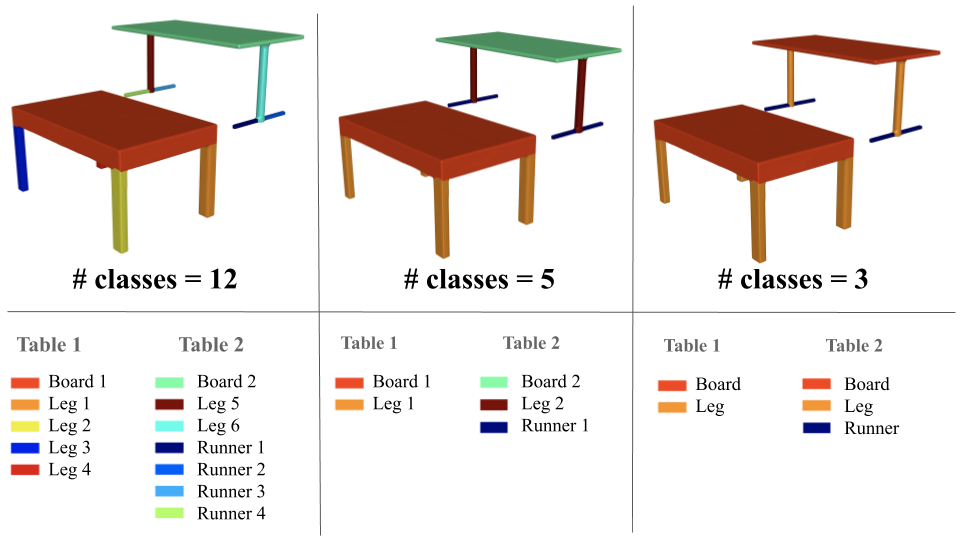
\includegraphics[width=0.9\textwidth]{images/three_tables}
\caption{Different rules for combining the part trees of all the objects. (left) if colors of all the legs are different, (center) if color of legs depends on the the table, (right) if color of all legs are the same. Instance information doesn't always provide relevant information about the part of the object, and is redundant in most samples.}
\end{figure}







\paragraph{Taxonomy statistics. }
\label{dataset:taxonomy-stats}
% say something about taxonomy 

% Under closer examination, we discovered that most of the parts do not have a unique shape making the task of instance segmentation for parts very hard to solve and not necessary for practical scene segmentation task. 



% Плюс учитывая то, что скидывал раньше Саша, supplementary должно состоять как минимум из следующего:
%  1. Детали датасета. Разные уровни разметки (есть), разные уровни агрегации (есть)
%  2. Детальное описание таксономии. Табличка “количество уровней в дереве” X “порог обрубания вершин”, в ячейках количество классов (есть), аргументация о выборе оптимального порога 1800 (нет), полная таксономия на трёх уровнях (есть).


Table~\ref{tab:taxonomy_structure_by_threshold} displays class statistics with taxobtained by thresholding at different values of the class occurrence. 

%  • [146] We proceed with this reduction by first choosing an appropriate occurrence threshold (we pick 1800 voxels, but demonstrate the effect of different threshold values in the supplementary) and remove classes that have smaller number of representatives in the dataset. — здесь необходимо привести табличку (количество уровней в дереве X порог обрубания вершин). Табличка посчитана, но непонятно, как из неё сделать вывод, что порог 1800 вокселей — оптимальный. @ чем ты руководствовался при выборе этого порога?

\begin{table}[!ht]
    \centering
    \caption{The effect of class occurrence threshold on taxonomy structure. For each depth $d_k$ in the PartNet taxonomy, we display the number of classes $|\mathbb{C}_k|$ with occurrence values greater than \#\,Voxels threshold (left column). The shaded row approximately corresponds to our taxonomy structure.}
    \begin{tabular}{r cccccccc}
        \toprule
        & \multicolumn{8}{c}{Depth $d_k$} \\
        \cmidrule{2-9}
        \#\,Voxels & 1 & 2 & 3 & 4 & 5 & 6 & 7 & 8 \\
         & (object) & (coarse) & & & & & & (fine) \\
        \midrule
        0    & 18 & 50 & 133 & 223 & 269 & 302 & 306 & 307 \\
        1K   & 15 & 42 &  86 & 119 & 142 & 147 & 152 & 156 \\
        \rowcolor{LightGray}
        2K   & 12 & 28 &  60 &  96 & 117 & 122 & 127 & 131 \\
        5K   & 11 & 21 &  43 &  70 &  86 &  89 &  93 &  97 \\
        10K  & 11 & 19 &  35 &  57 &  70 &  72 &  74 &  75 \\
        20K  &  8 & 15 &  26 &  43 &  50 &  51 &  52 &  52 \\
        50K  &  6 & 13 &  19 &  27 &  29 &  29 &  29 &  29 \\
        100K &  6 & 11 &  15 &  21 &  22 &  22 &  22 &  22 \\
        \bottomrule
    \end{tabular}
    \label{tab:taxonomy_structure_by_threshold}
\end{table}


% \VI{DONE: more figures displaying taxonomies for example objects (like Figure 1 in main text)}
%  5. Несколько дополнительных примеров пропажи лейблов в результате перехода PartNet -> Scannet (нет) (наподобие рисунка 1 основной статьи)

\begin{figure}[!t]
\label{fig:more_teasers}
\centering
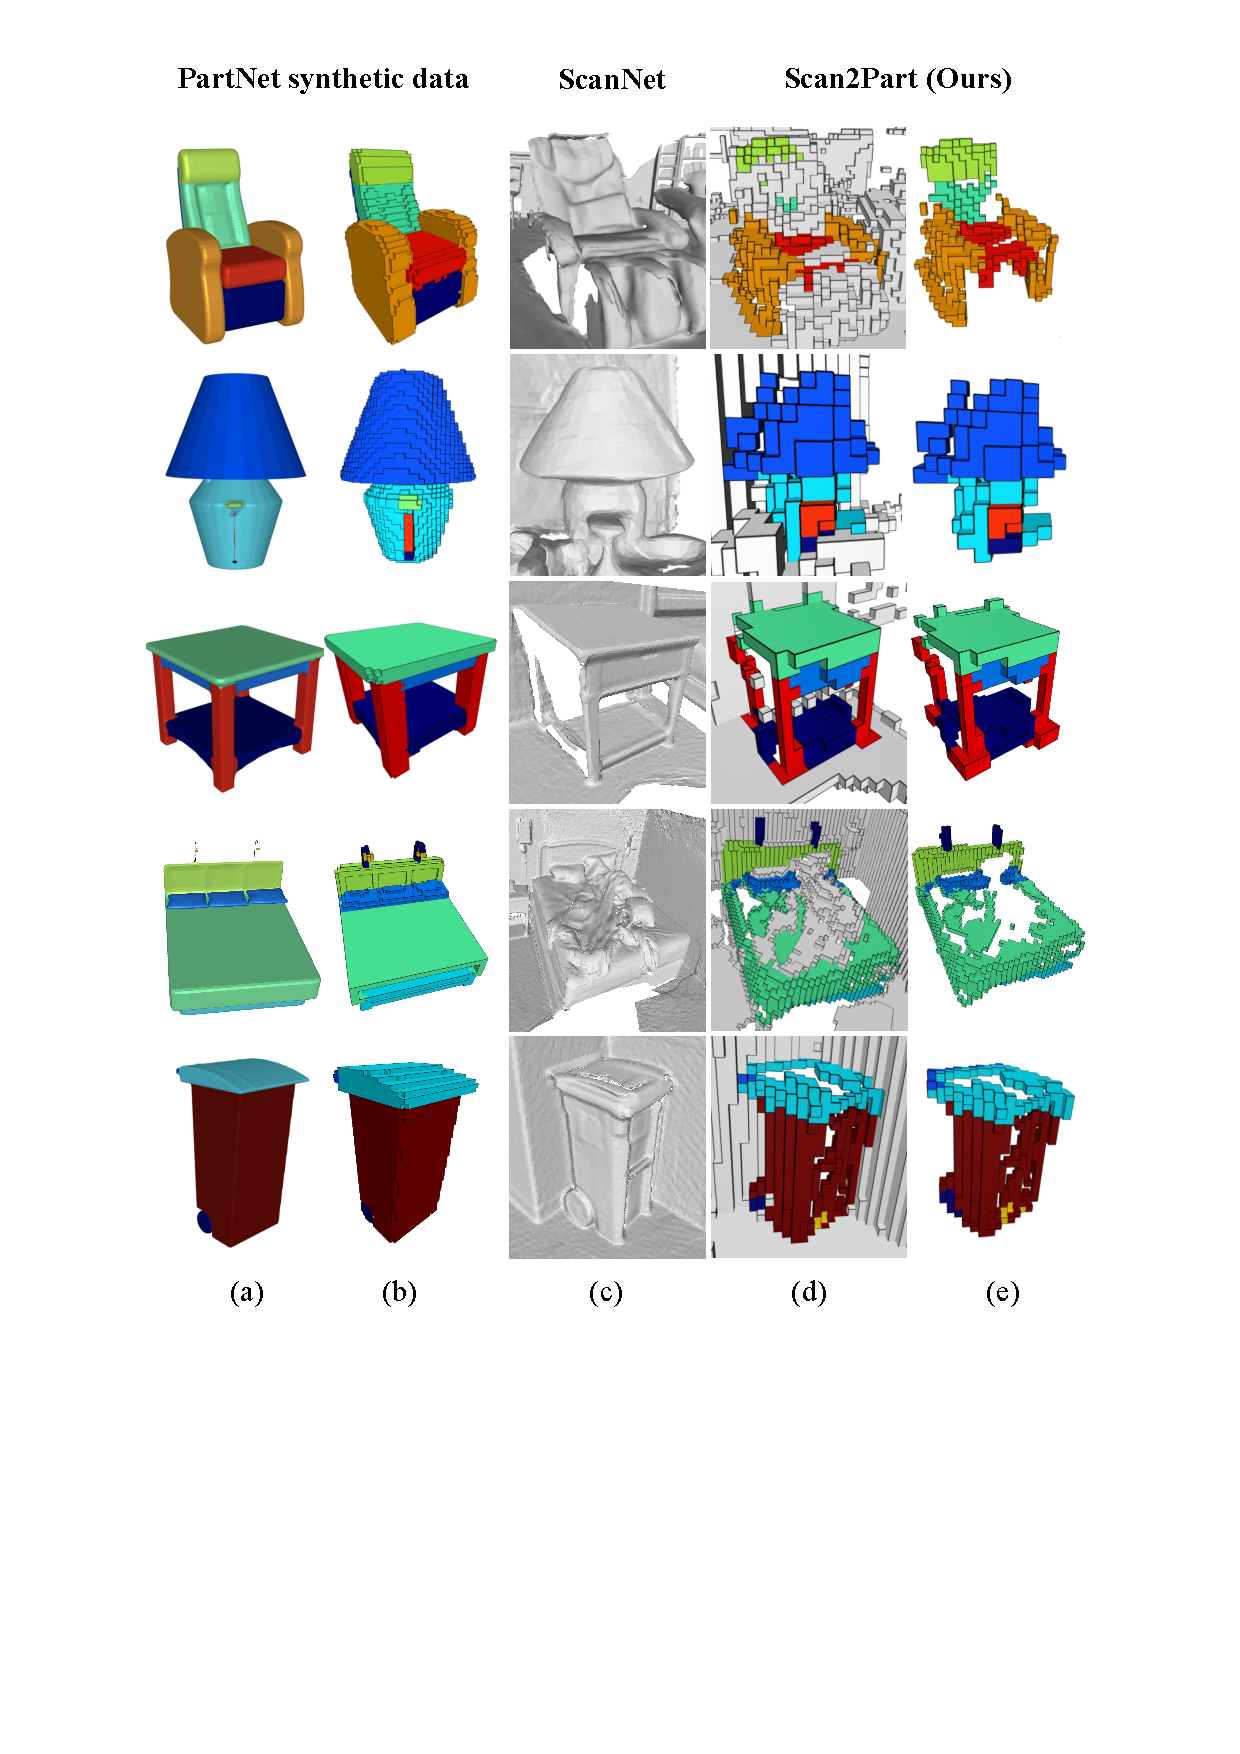
\includegraphics[width=\textwidth]{images/more_teasers.pdf}
\caption{Example voxelized shapes from our Scan2Part dataset. From left to right: 
(a) source 3D CAD model with part category annotations from PartNet~\cite{mo2019partnet},
(b) voxelized 3D shape with voxel-level parts annotation,
(c) fragment of reconstructed 3D scan geometry with a real-world instance of the same object,
(d) voxelized 3D scan geometry annotated according to our automatic procedure,
(e) real-world voxelized 3D shape (resolution $=3$\,cm$^3$) with voxel-level parts annotation.
Note the significant difference in geometry between synthetic and real-world volumetic 3D shapes due to noisy and incomplete geometry.}
\end{figure}


\begin{figure}[!t]
\label{fig:part_level_variation_voxels}
\centering
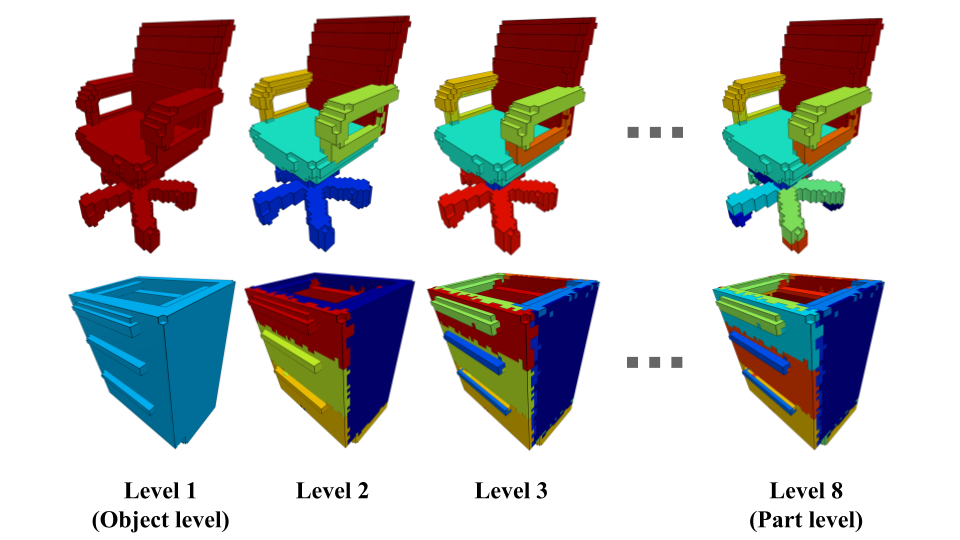
\includegraphics[width=\textwidth]{images/part_level_variation_voxels.png}
\caption{Example instances from our Scan2Part dataset, segmented according to level of detail depending on the part tree PartNet-based taxonomy~\cite{mo2019partnet}. The level of detail  increases from left to right, starting with the object level.}
\end{figure}

% \LA{figure displaying the taxonomy as a tree}
% VI: colored Treemap by AN

\begin{figure}[!t]
\label{fig:dataset_treemap}
\centering
% <left> <lower> <right> <upper>
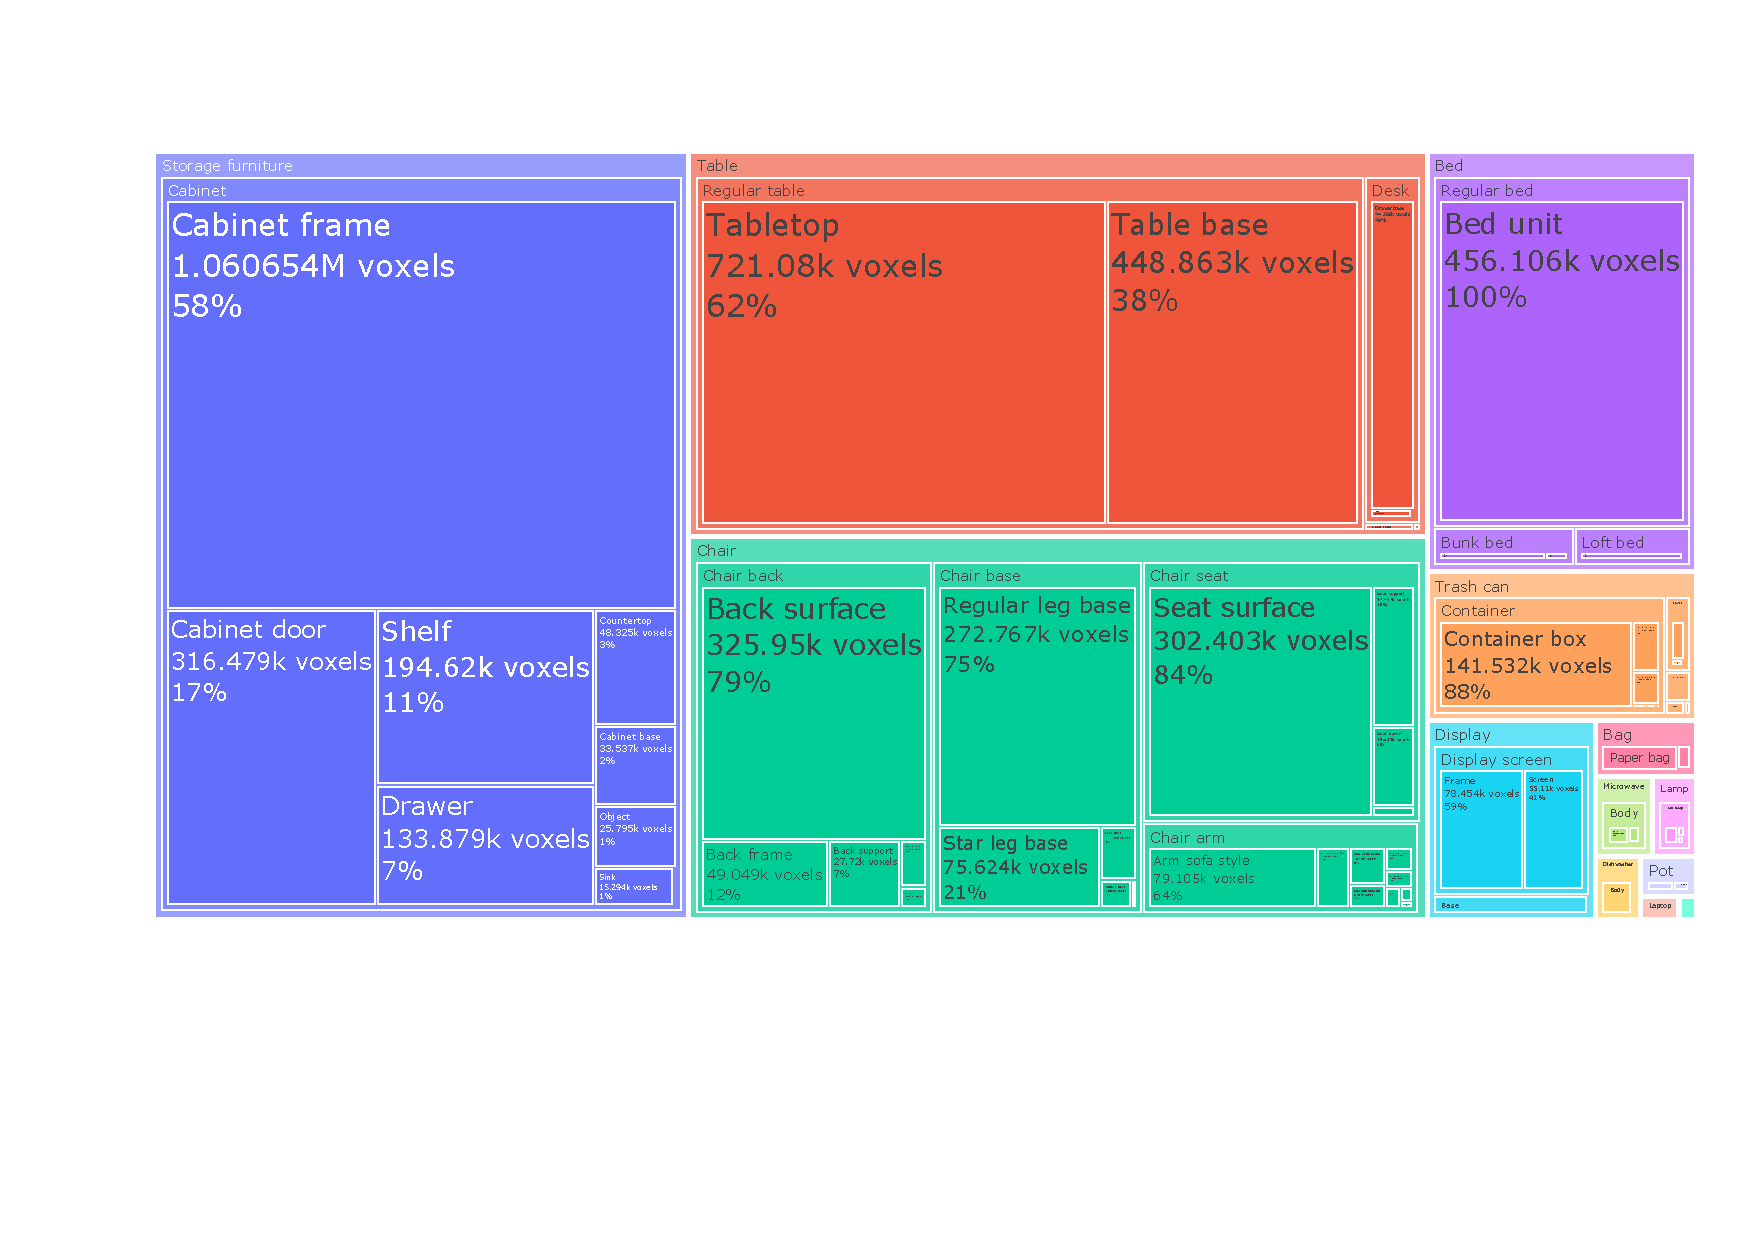
\includegraphics[trim={2.5cm 5cm 1cm 3cm},clip,width=\textwidth]{images/treemap_plot30px.pdf}
\caption{Statistics of Scan2Part dataset, area of tiles correspond to absolute number of voxels in the dataset}
\end{figure}


\paragraph{Dataset statistics. }
\label{dataset:statistics-detail}




% \begin{table}[!htb]
% \caption{Full dataset and testset statistics. As you can see it's highly unbalanced.}
% \resizebox{\textwidth}{!}{%
% \begin{tabular}{l|lllll}
% classes & \% in testset & \# voxel & \% voxels & \# scenes & \# inst. in testset\\ \hline
% Microwave & 18.75\% & 20141 & 0.38\% & 90 & 21\\
% Display & 19.36\% & 149988 & 2.84\% & 350 & 142\\
% Lamp & 20.14\% & 15736 & 0.30\% & 95 & 26\\
% Laptop & 19.95\% & 3950 & 0.07\% & 46 & 11\\
% Bag & 19.75\% & 25225 & 0.48\% & 136 & 33\\
% Storage & 19.41\% & 1833826 & 34.68\% & 866 & 496\\
% Bed & 20.94\% & 504774 & 9.55\% & 271 & 69\\
% Table & 20.82\% & 1268401 & 23.99\% & 1104 & 539\\
% Chair & 16.95\% & 1261928 & 23.87\% & 960 & 754\\
% Dishwasher & 20.99\% & 12846 & 0.24\% & 24 & 6\\
% TrashCan & 18.96\% & 178648 & 3.38\% & 634 & 199\\
% Vase & 20.48\% & 9989 & 0.19\% & 30 & 9\\
% Keyboard & 19.63\% & 1819 & 0.03\% & 24 & 9\\
% % Bowl & 28.86\% & 1178 & 0.02\% & 12 \\
% % Faucet & 2.44\% & 246 & 0.00\% & 4 \\
% % Clock & 12.28\% & 1742 & 0.03\% & 15 \\
% % Hat & 100.00\% & 101 & 0.00\% & 1 \\
% % Bottle & 0.00\% & 23 & 0.00\% & 1
% \end{tabular}%
% \label{tab:datasetstats}
% }
% \end{table}



% \begin{table}[hbt]
% \caption{Proportions of ShapeNet semantic classes present in Scan2Cad dataset}
% \label{table:scan2part_proportions}
% \begin{tabular}{l|l|l}
% Class ID & overlap? & class name \\
% \hline
% 04379243 & 99.0\% (822/830) & table \\ \hline
% 02747177 & 98.9\% (88/89) & ashcan,trash can,garbage can,wastebin,ash bin,ash-bin \\ \hline
% 03211117 & 97.6\% (161/165) & display,video display \\ \hline
% 03761084 & 97.3\% (36/37) & microwave,microwave oven \\ \hline
% 03337140 & 97.1\% (68/70) & file,file cabinet,filing cabinet \\ \hline
% 03001627 & 96.9\% (632/652) & chair \\ \hline
% 02871439 & 96.7\% (145/150) & bookshelf \\ \hline
% 02933112 & 94.8\% (294/310) & cabinet \\ \hline
% 02818832 & 94.0\% (47/50) & bed \\ \hline
% 03991062 & 91.7\% (11/12) & pot,flowerpot \\ \hline
% 03207941 & 85.7\% (12/14) & dishwasher,dish washer,dishwashing machine \\ \hline
% 03085013 & 81.8\% (9/11) & computer keyboard,keypad \\ \hline
% 03325088 & 57.1\% (4/7) & faucet,spigot \\ \hline
% 02876657 & 50.0\% (1/2) & bottle \\ \hline
% 02808440 & 26.0\% (25/96) & bathtub,bathing tub,bath,tub \\ \hline
% 02801938 & 9.4\% (3/32) & basket,handbasket \\ \hline
% 04256520 & 8.1\% (20/247) & sofa,couch,lounge \\ \hline
% 02946921 & 0.0\% (0/1) & can,tin,tin can \\ \hline
% 03938244 & 0.0\% (0/5) & pillow \\ \hline
% 02828884 & 0.0\% (0/28) & bench \\ \hline
% 04554684 & 0.0\% (0/37) & washer,automatic washer,washing machine \\ \hline
% 03928116 & 0.0\% (0/25) & piano,pianoforte,forte-piano \\ \hline
% 03790512 & 0.0\% (0/4) & motorcycle,bike \\ \hline
% 03691459 & 0.0\% (0/2) & loudspeaker,speaker,speaker unit,loudspeaker system \\ \hline
% 03467517 & 0.0\% (0/6) & guitar \\ \hline
% 04330267 & 0.0\% (0/36) & stove \\ \hline
% 04401088 & 0.0\% (0/1) & telephone,phone,telephone set \\ \hline
% 04004475 & 0.0\% (0/31) & printer,printing machine \\ \hline
% Total:    & 81.2\% (2477/3049) &         \\
% \end{tabular}
% \end{table}

